%%%%%%%%%%%%%%%%%%%%%%%%%%%%%%%%%%%%%%%%%%%%%%%%%%%%%%%%%%%%%%%%%%%%%%%%%%%
\section{\label{sec:Contrib-Info}Introduction}
%%%%%%%%%%%%%%%%%%%%%%%%%%%%%%%%%%%%%%%%%%%%%%%%%%%%%%%%%%%%%%%%%%%%%%%%%%%

Contrib modules are stand alone, separate pieces of code that work
together with Condor to accomplish some task.
These modules are available for download at 
\URL{http://research.cs.wisc.edu/condor/downloads-v2}.
Documentation for these modules is either here and identified
as a contrib module, 
or may be within the module itself.

Other features of Condor are available within the source code,
but are not compiled in to the binaries distributed.
To utilize these features, 
acquire the source code and build it.
Enable the feature as described in this documentation.

This chapter documents the CondorView Client contrib module,
Quill (available with the source code),
and using Condor with the Hadoop File System (available with the source code).


%%%%%%%%%%%%%%%%%%%%%%%%%%%%%%%%%%%%%%%%%%%%%%%%%%%%%%%%%%%%%%%%%%%%%%%%%%%
\subsection{\label{sec:Condor-HDFS}Using Condor with the Hadoop File System}
%%%%%%%%%%%%%%%%%%%%%%%%%%%%%%%%%%%%%%%%%%%%%%%%%%%%%%%%%%%%%%%%%%%%%%%%%%%
\index{Hadoop Distributed File System (HDFS)!integrated with Condor}

The Hadoop project is an apache project, headquartered at http://hadoop.apache.org, 
which implements an open-source, distributed filesystem across a large set
of machines.  The file system proper is called the Hadoop File System, or hdfs, and 
there are several hadoop-provided tools which use the file system, most notably
databases and tools which use the map-reduce distributed programming style.  Condor
provides a way to manage the daemons which implement hadoop file system, but no
direct support for the high-level tools which run atop this file system.  There
are two types of daemons which together create an instance of a hadoop filesystem.
The first is called the Name Node, which is like the central manager for a 
hadoop cluster.  There is only one active Name Node per hadoop filesystem.  If
the Name node is not running, no files can be accessed.  Hadoop does not support
failover of the name node, but does support a hot-spare for the name node, called
the backup node.  Condor can configure one node to be running as a backup name node.
The second
kind of daemon is the Data node, and there is one data node per machine in the 
distributed filesystem.  As these are both implemented in Java, Condor cannot directly
manage these daemons.  Rather, we provide a small daemon-core daemon, called
condor\_hdfs which reads the condor config file, responds to condor commands like
condor\_on and condor\_off, and runs the Hadoop java code.  It translates entries
in the condor config file to an XML format native to condor.  These configuration
items are listed with the condor\_hdfs daemon in section~\ref{sec:HDFS-Config-File-Entries}. 
So, to configure HDFS in condor, the condor config file should specify one machine in the
pool to be the HDFS name node, and others to be the data node.

Once an HDFS is deployed, condor jobs can directly use it in a vanilla universe job, by transfering input files directly from the HDFS by specifying a URL within the
job's \SubmitCmd{transfer\_input\_files} command. 
See section~\ref{sec:URL-transfer} for the administrative details
to set up transfers specified by a URL.
It requires that a plug-in is accessible and defined to handle
\Expr{hdfs} protocol transfers. 


%%%%%%%%%%%%%%%%%%%%%%%%%%%%%%%%%%%%%%%
\section{\label{sec:Quill}Quill}
%%%%%%%%%%%%%%%%%%%%%%%%%%%%%%%%%%%%%%%
\index{Quill|(}

Quill builds and maintains a mirror database of a Condor job queue.
The \Condor{quill} daemon implements it,
and the \Condor{q} and \Condor{history} tools use it.

%%%%%%%%%%%%%%%%%%%%%%%%%%%%%%%%%%%%%%%
\subsection{\label{sec:Quill-Installation}Installation and Configuration}
%%%%%%%%%%%%%%%%%%%%%%%%%%%%%%%%%%%%%%%

Quill uses the \Prog{PostgreSQL} database management system.
Quill uses the \Prog{PostgreSQL} server as its back end
and client library, 
\Prog{libpq} to talk to the server.
Quill works with \Prog{PostgreSQL}
version 8.0;
it has also been tested with version 7.4.

Obtain \Prog{PostgreSQL} from

\URL{http://www.postgresql.org/ftp/source/}

Installation instructions are detailed in:
\URL{http://www.postgresql.org/docs/8.0/static/installation.html}

Configure \Prog{PostgreSQL} after installation:

\begin{enumerate}
\item The \Condor{quill} daemon and client tools connect
to the database as users \Username{quillreader} and 
\Username{quillwriter}.
These are database users, not operating system users.
The two types of users are quite different from each other.
If these data base users do not exist,
add them using the 
\Prog{createuser} command supplied with the installation.
Assign them with appropriate passwords;
these passwords will be used by the Quill tools to connect
to the database in a secure way.
User \Username{quillreader} should not be allowed to create
more databases nor create more users.
User \Username{quillwriter} should
not be allowed to create more users,
however it should be allowed to create more databases.
The following commands create the two users
with the appropriate permissions,
and be ready to enter the corresponding passwords when prompted.

\footnotesize
\begin{verbatim}
/path/to/postgreSQL/bin/directory/createuser quillreader \
	--no-createdb --no-adduser --pwprompt

/path/to/postgreSQL/bin/directory/createuser quillwriter \
	--createdb --no-adduser --pwprompt
\end{verbatim}
\normalsize


\item Configure to accept TCP/IP connections.
For \Prog{PostgreSQL} version 8,
use the \Code{listen\_addresses} variable in 
\File{postgresql.conf} file as a guide.
For example,
\Code{listen\_addresses = '*'}
means listen on any IP interface.
In \Prog{PostgreSQL} version 7,
this was accomplished by setting 
\Code{tcpip\_socket=true} in the \File{postgresql.conf} file.


\item Configure \Prog{PostgreSQL} to accept TCP/IP connections from 
specific hosts.
Modify the \File{pg\_hba.conf} file 
(which usually resides in the \Prog{PostgreSQL} server's data directory).
Access is required by the \Condor{quill} daemon,
as well as the database users
\Username{quillreader} and \Username{quillwriter}.
For example, to give
database users \Username{quillreader} and \Username{quillwriter}
password-enabled access to all databases on current machine from any
other machine in the network, add the following:

\begin{tabular}{llllll}
host&all&quillreader&128.105.0.0&255.255.0.0&password\\
host&all&quillwriter&128.105.0.0&255.255.0.0&password
\end{tabular}

Note that in addition to the database specified by
the configuration variable \MacroNI{QUILL\_DB\_NAME},
the \Condor{quill} daemon also needs access to the database
"template1".
In order to create the database in the first place, 
the \Condor{quill} daemon needs to connect to the database.

\item The \Condor{quill} daemon needs read and write access
to the database.
It connects as user \Username{quillwriter},
who has owner privileges to the database.
Since this gives all access to the \Username{quillwriter} user,
this password cannot be stored in a public place 
(such as the \Condor{collector}).
For this reason, the \Username{quillwriter} password is stored
in a file named \File{.quillwritepassword} in the Condor spool directory.
Appropriate protections on this file guarantee secure access to the database.
This file must be created and protected by the site administrator;
if this file does not exist as and where expected, the \Condor{quill}
daemon logs an error and exits.

\end{enumerate}


Condor must also be configured to use Quill.

\begin{description}
\item Add \Expr{QUILL} to the variable \MacroNI{DAEMON\_LIST}.
\item Add the file \File{.quillwritepassword} to the 
  \MacroNI{VALID\_SPOOL\_FILES} variable, since \Condor{preen} must
  be told not to delete this file.
\item Tell Condor where Quill resides, as well as specify Quill's
  start-up arguments:
\begin{verbatim}
QUILL = $(SBIN)/condor_quill
QUILL_ARGS = -f
\end{verbatim}
\item Identify Quill's log file:
\begin{verbatim}
QUILL_LOG = $(LOG)/QuillLog
\end{verbatim}
\item Set up all other configuration variables that are specific
  to the installation.
\footnotesize
\begin{verbatim}
QUILL_ENABLED           = TRUE
QUILL_NAME              = some-unique-quill-name.cs.wisc.edu
QUILL_DB_NAME           = database-for-some-unique-quill-name
QUILL_DB_IP_ADDR        = databaseipaddress:port
# the following parameter's units is in seconds
QUILL_POLLING_PERIOD    = 10
# the following parameter's units is in hours
QUILL_HISTORY_CLEANING_INTERVAL = 24
# the following parameter's units is in days
QUILL_HISTORY_DURATION 	= 30
QUILL_IS_REMOTELY_QUERYABLE = TRUE
QUILL_DB_QUERY_PASSWORD =  password-for-database-user-quillreader
QUILL_ADDRESS_FILE      = $(LOG)/.quill_address
\end{verbatim}
\normalsize

\end{description}


Descriptions of these and other configuration variables are in
section~\ref{sec:Quill-Config-File-Entries}.
Here are further brief details:

\begin{itemize}

\item \Macro{QUILL\_DB\_<NAME>} and \Macro{QUILL\_DB\_IP\_ADDR}\\
These two variables are used to determine the location of the database
server that this Quill would talk to, and the name of the database that
it creates.  More than one Quill server can talk to the same database
server.  This can be done by simply letting all the 
\MacroNI{QUILL\_DB\_IP\_ADDR} point to the same database server.

If more than one Quill server are sharing the same database
server, then the \MacroNI{QUILL\_DB\_NAME} variable for all of them should
be unique.  Otherwise, there would be record overwriting and corruption
of job queue information.

\item \Macro{QUILL\_POLLING\_PERIOD}\\
This controls the frequency with which Quill polls the
\File{job\_queue.log} file.  By default, it is 10 seconds.  Since Quill
works by periodically sniffing the log file for updates and then sending
those updates to the database, this variable controls the trade off between
the currency of query results and Quill's load on the system--usually
negligible.

\item \Macro{QUILL\_HISTORY\_CLEANING\_INTERVAL} and 
		\Macro{QUILL\_HISTORY\_DURATION}\\
These two variables control the deletion of historical jobs from the
database.  \MacroNI{QUILL\_HISTORY\_DURATION} is the number of days
after completion (more precisely, the number of days since the history ad got 
into the history database - those two might be different if a job is completed 
but stays in the queue for a while) that a given job will stay in the database.  
So all jobs beyond \MacroNI{QUILL\_HISTORY\_DURATION} will be deleted.  Now,
scanning the entire database for old jobs can get pretty expensive,
so the other variable \MacroNI{QUILL\_HISTORY\_CLEANING\_INTERVAL}
is the number of hours between two successive scans.  By default,
\MacroNI{QUILL\_HISTORY\_DURATION} is set to 180 days and
\MacroNI{QUILL\_HISTORY\_CLEANING\_INTERVAL} is set to 24 hours.

\item \Macro{QUILL\_IS\_REMOTELY\_QUERYABLE}\\
Thanks to 
\Prog{PostgreSQL},
one can now remotely query both the job queue and the
history tables. This variable controls whether this remote querying 
feature should be enabled.  By default it is TRUE.  Note that even if 
this is FALSE, one can still query the job queue in the remote schedd
This variable only controls whether the database tables are remotely queryable.

\item \Macro{QUILL\_DB\_QUERY\_PASSWORD}\\
In order for the query tools to connect to a database, it needs to provide
the password that is assigned to database user \Username{quillreader}. 
This variable is then advertised by the \Condor{quill} daemon
to the \Condor{collector}.  
This facility enables remote querying: remote \Condor{q} query tools first 
ask the \Condor{collector} for the password associated with a particular Quill database 
and then query that database.  Users who do not have access to the collector 
cannot view the password and as such cannot query the database.  Again, this 
password just provides 'read' access to the database.

\item \Macro{QUILL\_ADDRESS\_FILE}\\
When Quill starts up, it can place it's address (IP and port)
into a file.  This way, tools running on the local machine do not
need to query the central manager to find Quill.  This 
feature can be turned off by commenting out the variable.

\end{itemize}


%%%%%%%%%%%%%%%%%%%%%%%%%%%%%%%%%%%%%%%
\subsection{\label{sec:Quill-Example}Four Usage Examples}
%%%%%%%%%%%%%%%%%%%%%%%%%%%%%%%%%%%%%%%


\begin{enumerate}
\item Query a remote Quill daemon on \File{regular.cs.wisc.edu}
for all the jobs in the queue
\begin{verbatim}
	condor_q -name quill@regular.cs.wisc.edu
	condor_q -name schedd@regular.cs.wisc.edu

\end{verbatim}
There are two ways to get to a Quill daemon: directly using its name as 
specified in the \MacroNI{QUILL\_NAME} configuration variable, or indirectly
by querying the \Condor{schedd} daemon using its name.
In the latter case, \Condor{q} will detect 
if that \Condor{schedd} daemon is being serviced by a database, and if so, directly query it.
In both cases, the IP address and port of the database server hosting the data of 
this particular remote Quill daemon can be figured out by the \MacroNI{QUILL\_DB\_IP\_ADDR} 
and \MacroNI{QUILL\_DB\_NAME} variables specified in the \MacroNI{QUILL\_AD}
sent by the quill daemon to the collector and in the \MacroNI{SCHEDD\_AD} sent by
the \Condor{schedd} daemon.  

\item Query a remote Quill daemon on \File{regular.cs.wisc.edu} for all historical 
jobs belonging to owner einstein.
\begin{verbatim}
	condor_history -name quill@regular.cs.wisc.edu einstein
\end{verbatim}

\item Query the local Quill daemon for the average time spent in the queue 
for all non-completed jobs. 
\begin{verbatim}
	condor_q -avgqueuetime 
\end{verbatim}
The averate queue time is defined as the average of
\Expr{(currenttime - jobsubmissiontime)} over all jobs which are neither
completed \Expr{(JobStatus == 4)} or removed \Expr{(JobStatus == 3)}.

\item Query the local Quill daemon for all historical jobs completed since 
Apr 1, 2005 at 13h 00m.
\begin{verbatim}
	condor_history -completedsince '04/01/2005 13:00'
\end{verbatim}
It fetches all jobs
which got into the 'Completed' state on or after the
specified time stamp.  It use the \Prog{PostgreSQL} date/time
syntax rules, as it encompasses most format options.  See
\URL{http://www.postgresql.org/docs/8.0/static/datatype-datetime.html\#AEN4516}
for the various time stamp formats.

\end{enumerate}

%%%%%%%%%%%%%%%%%%%%%%%%%%%%%%%%%%%%%%%
\subsection{\label{sec:Quill-Schema}Quill and Its RDBMS Schema}
%%%%%%%%%%%%%%%%%%%%%%%%%%%%%%%%%%%%%%%

With only 7 tables and 2 views, Quill uses a relatively simple database
schema.  These can be broadly divided into tables used to store job
queue information and those used to store historical information.

The job queue part of the schema closely follows Condor's ClassAd data
model. For example, each row in these tables describe an <attribute,value>
pair of the classad.  Additionally, just as how Condor distinguishes a
ClusterAd from a ProcAd where the former stores attributes common to all
jobs within a cluster whereas the latter stores attributes specific to
each job, the schema also makes this distinction.  Finally, numerical
and string valued attributes are stored separately.

Thus, there are four tables:

\begin{itemize}

\item 
	\SQLTableDef{ClusterAds\_Str}
		{cid int, 
		attr text, 
		val text, 
		primary key (cid, attr)}

\item 
	\SQLTableDef{ClusterAds\_Num}
		{cid int, 
		attr text, 
		val double precision, 
		primary key (cid, attr)}

\item 
	\SQLTableDef{ProcAds\_Str}
		{cid int, 
		pid int, 
		attr text, 
		val text, 
		primary key (cid, pid, attr)}

\item 
	\SQLTableDef{ProcAds\_Num}
		{cid int, 
		pid int, 
		attr text, 
		val double precision,
		primary key (cid, pid, attr)}

\end{itemize}

In addition to the <attribute, value>, each row contains the cluster-id
(cid) and in the case of the ProcAd tables, also the proc-id (pid).

Since each ClassAd would be split into potentially two tables (string
and numeric), there are views that unify them into a single entity in
order to simplify queries.

Here are the view definitions:

\begin{itemize}
\item Definition of ClusterAds view\\
	\SQLViewDef{ClusterAds}
		{select cid, 
		attr, 
		val from ClusterAds\_Str UNION ALL
		select cid, 
		attr, 
		cast(val as text) from ClusterAds\_Num}


\item Definition of ProcAds view\\
	\SQLViewDef{ProcAds}
		{select cid, 
		pid, 
		attr, 
		val from ProcAds\_Str UNION ALL
		select cid, 
		pid, 
		attr, 
		cast(val as text) from ProcAds\_Num}

\end{itemize}

Finally, the job queue part of the schema also contains a table that
stores metadata information related to the \File{job\_queue.log} file.

\begin{itemize}
\item \SQLTableDef{JobQueuePollingInfo}
        {last\_file\_mtime         BIGINT,
        last\_file\_size          BIGINT,
        last\_next\_cmd\_offset    BIGINT,
        last\_cmd\_offset         BIGINT,
        last\_cmd\_type           SMALLINT,
        last\_cmd\_key            text,
        last\_cmd\_mytype         text,
        last\_cmd\_targettype     text,
        last\_cmd\_name           text,
        last\_cmd\_value          text}
\end{itemize}
	
At all times, there is only 1 row in this table and it describes
information related to the last time Quill polled the \File{job\_queue.log} file.

\begin{itemize}
\item \Bold{last\_file\_mtime} and \Bold{last\_file\_size}\\
	The last modified time and size of the file.

\item \Bold{last\_cmd\_offset} and \Bold{last\_next\_cmd\_offset}\\
	The offsets of the record last read from the file and its successive record.

\item \Bold{last\_cmd\_type}\\
	The command type (101, 102, etc.) of the record.

\item	\Bold{last\_cmd\_key}, 
		\Bold{last\_cmd\_mytype}, 
		\Bold{last\_cmd\_targettype},
		\Bold{last\_cmd\_name},
		and
		\Bold{last\_cmd\_value}\\
	Together, these attributes define the record itself.	The key
	refers to the combined "cid.pid" pair, mytype and target usually
	contains Job and Machine respectively, and finally the name and
	value contains the <attribute,value> pair.
\end{itemize}

The historical information on the other hand is slightly differently
designed.  Instead of a purely vertical data model (each row is a
$<$attribute,value$>$ pair), we have two tables that together represent the
complete job classad.  Their schema is as follows:

\begin{enumerate}

\item \SQLTableDef{History\_Horizontal}
        {cid                  int,
        pid                  int,
	EnteredHistoryTable  timestamp with time zone,
        Owner                text,
        QDate                int,
        RemoteWallClockTime  int,
        RemoteUserCpu        float,
        RemoteSysCpu         float,
        ImageSize            int,
        JobStatus            int,
        JobPrio              int,
        Cmd                  text,
        CompletionDate       int,
        LastRemoteHost       text,
        primary key(cid,pid)}

\item \SQLTableDef{History\_Vertical}
	{cid int, pid int, attr text, val text, primary key
	(cid, pid, attr)}

\end{enumerate}

Each historical job ad is divided into its horizontal and vertical
counterparts.  This division was made because of query performance
reasons.  While its easier to store ClassAds in a vertical table,
queries on vertical tables generally perform worse than those on
horizontal tables since the latter has lot fewer records.  However, in
Condor, since job ads do not have a fixed schema (users can define their
own attributes), a purely horizontal schema would end up having a lot
of null values. As such, we have a hybrid schema where attributes on
which queries are frequently performed (via \Condor{history}) are put
in the \SQLTable{History\_Horizontal} table and the other attributes
are stored vertically (just as in the Cluster/Proc tables above) in the
\SQLTable{History\_Vertical} table. Also \SQLTable{History\_Horizontal}
contains all the attributes needed to service the short form of the
\Condor{history} command (that is, without the -l option).

The resulting hybrid schema has proven to be the most efficient in
servicing \Condor{history} queries.  The job queue tables (Cluster and
Proc) were not designed in this hybrid manner because job queues aren't
as large as history; just a vertical schema worked great.


%%%%%%%%%%%%%%%%%%%%%%%%%%%%%%%%%%%%%%%
\subsection{\label{sec:Quill-Security}Quill and Security}
%%%%%%%%%%%%%%%%%%%%%%%%%%%%%%%%%%%%%%%

There are several layers of security in Quill, some provided by Condor and
others provided by the database.  First, all accesses to the database
are password-protected.

\begin{enumerate}
\item The query tools, \Condor{q} and
\Condor{history} connect to the database as user \Username{quillreader}.
The password for this user can vary from one database to another and
as such, each Quill daemon advertises this password to the collector.
The query tools then obtain this password from the collector and
connect successfully to the database.  Access to the database by the
\Username{quillreader} user is read-only, as this is sufficient for the
query tools.  The \Condor{quill} daemon ensures this protected access using the sql
GRANT command when it first creates the tables in the database.  Note that
access to the \Username{quillreader} password itself can be blocked by
blocking access to the collector, a feature already supported in Condor.

\item The \Condor{quill} daemon, on the other hand, needs read and write access
to the database.  As such, it connects as user \Username{quillwriter},
who has owner privileges to the database.  Since this gives all
access to the \Username{quillwriter} user, this password cannot
be stored in a public place (such as the collector).  For this
reason, the \Username{quillwriter} password is stored in a file called
\File{.quillwritepassword} in the Condor spool directory.
Appropriate protections on this file guarantee secure access to the database.
This file must be created and protected by the site administrator;
if this file does not exist as and where expected, the \Condor{quill}
daemon logs an error and exits.

\item The \Attr{IsRemotelyQueryable} attribute in the Quill ClassAd advertised
by the Quill daemon to the collector can be used by site administrators
to disallow the database from being read by all remote Condor query tools.

\end{enumerate}


%%%%%%%%%%%%%%%%%%%%%%%%%%%%%%%%%%%%%%%%%%%%%%%%%%%%%%%%%%%%%%%%%%%%%%
\section{\label{sec:HTCondorView-Client-Install}
The HTCondorView Client Contrib Module} 
%%%%%%%%%%%%%%%%%%%%%%%%%%%%%%%%%%%%%%%%%%%%%%%%%%%%%%%%%%%%%%%%%%%%%%
\index{HTCondorView!Client}
\index{contrib module!HTCondorView client}

The HTCondorView Client contrib module is used to automatically generate
World Wide Web pages to display usage statistics of an HTCondor
pool.
Included in the module is a shell script which invokes the \Condor{stats}
command to retrieve pool usage statistics from the HTCondorView server, and
generate HTML pages from the results.  
Also included is a Java applet, which graphically visualizes HTCondor 
usage information.  
Users can interact with the applet to customize the visualization and to
zoom in to a specific time frame.
Figure~\ref{fig:view-screenshot} on page~\pageref{fig:view-screenshot}
is a screen shot of a web page created by HTCondorView.  
%  link gone, and script is not working Dec 2012
%To get a further feel for what pages generated by HTCondorView look like,
%view the statistics for the University of Wisconsin-Madison pool 
%by visiting the URL 
%\URL{http://condor-view.cs.wisc.edu/condor-view-applet}.

\begin{figure}[hbt]
\centering
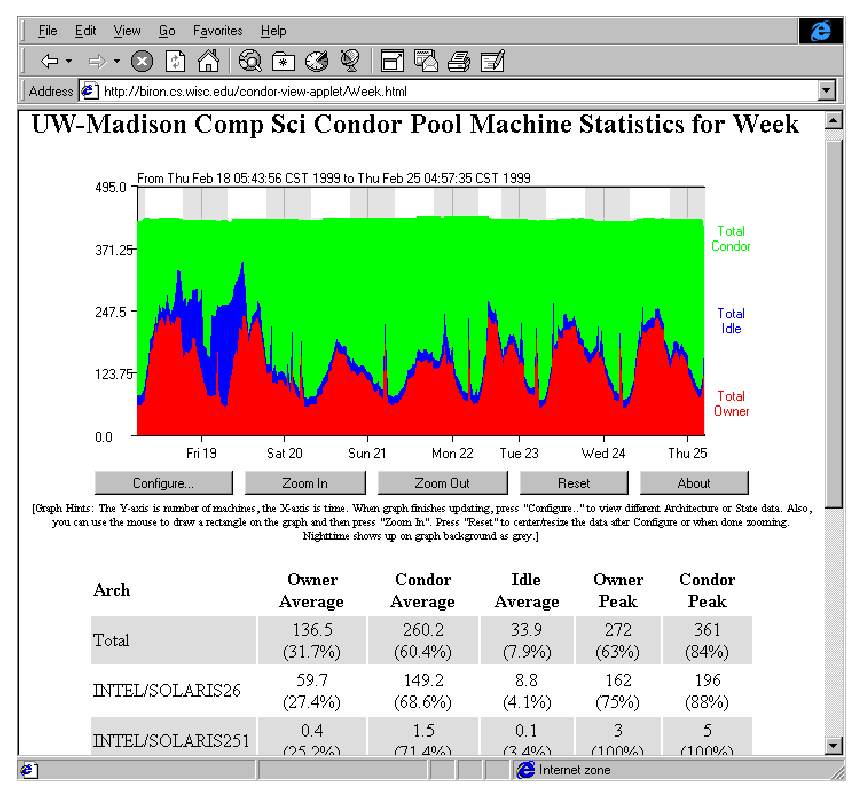
\includegraphics{contrib/view-screenshot.ps}
\caption{\label{fig:view-screenshot}Screen shot of HTCondorView Client}
\end{figure}

After unpacking and installing the HTCondorView Client, a script named
\Prog{make\_stats} can be invoked to create HTML pages displaying HTCondor usage
for the past hour, day, week, or month.  
By using the Unix \Prog{cron} facility to periodically execute
\Prog{make\_stats}, HTCondor pool usage statistics can be kept up to date
automatically.  
This simple model allows the HTCondorView Client to be easily installed;
no Web server CGI interface is needed.

%%%%%%%%%%%%%%%%%%%%%%%%%%%%%%%%%%%%%%%%%%%%%%%%%%%%%%%%%%%%%%%%%%%%%%
\subsection{\label{sec:condorview-client-step-by-step}
Step-by-Step Installation of the HTCondorView Client}
%%%%%%%%%%%%%%%%%%%%%%%%%%%%%%%%%%%%%%%%%%%%%%%%%%%%%%%%%%%%%%%%%%%%%%

\index{installation!HTCondorView Client}
\index{HTCondorView!Client installation}
\begin{enumerate}

\item Make certain that the HTCondorView Server is configured.
Section ~\ref{sec:Contrib-HTCondorView-Install}
describes configuration of the server.
The server logs information on disk in order to provide a persistent,
historical database of pool statistics.
The HTCondorView Client makes queries over the network to this
database.
The \Condor{collector} includes this database support.
To activate the persistent database logging, add the following entries to
the configuration file for the \Condor{collector} chosen to act as the ViewServer.
\begin{verbatim}
    POOL_HISTORY_DIR = /full/path/to/directory/to/store/historical/data 
    KEEP_POOL_HISTORY = True 
\end{verbatim}

\item Create a directory where HTCondorView is to place the HTML files.  
This directory should be one published by a web server, so that HTML
files which exist in this directory can be accessed using a web browser.  
This directory is referred to as the \File{VIEWDIR} directory.

\item Download the \Prog{view\_client} contrib module.
Follow links for contrib modules from the wiki at
\URL{https://htcondor-wiki.cs.wisc.edu/index.cgi/wiki}.

\item Unpack or untar this contrib module into the
directory \File{VIEWDIR}.
This creates several files and subdirectories.
Further unpack the jar file within the \File{VIEWDIR} directory with:
\begin{verbatim} 
  jar -xf condorview.jar
\end{verbatim}

\item Edit the \Prog{make\_stats} script.  At the beginning of the file
are six parameters to customize.
The parameters are

        \begin{description}

	\item[\MacroNI{ORGNAME}] A brief name that identifies an
	organization. An example is ``Univ of Wisconsin''.  Do not
	use any slashes in the name or other special regular-expression
	characters. Avoid the characters \Bs \^\  and \$.

	\item[\MacroNI{CONDORADMIN}] The e-mail
	address of the HTCondor administrator at your site.  
	This e-mail address will appear at the bottom of the web pages.

	\item[\MacroNI{VIEWDIR}] The full path name
	(\emph{not} a relative path) to the \File{VIEWDIR} directory set
	by installation step 2.  
	It is the directory that contains the \Prog{make\_stats} script.

	\item[\MacroNI{STATSDIR}]  The full path name of the
	directory which contains the \Condor{stats} binary.
	The \Condor{stats} program is included in the \Release{bin}
	directory. 
	The value for \MacroNI{STATSDIR} is added to the \MacroNI{PATH}
	parameter by default.  

	\item[\MacroNI{PATH}] A list of subdirectories,
	separated by colons, where the \Prog{make\_stats} script can find
	the \Prog{awk}, \Prog{bc}, \Prog{sed}, \Prog{date}, and \Condor{stats}
	programs.  
	If \Prog{perl} is installed, the path should also
	include the directory where \Prog{perl} is installed.
	The following default works on most systems:
        \begin{verbatim} 
        PATH=/bin:/usr/bin:$STATSDIR:/usr/local/bin
        \end{verbatim}

        \end{description}

\item To create all of the initial HTML files, run
\begin{verbatim}
        ./make_stats setup  
\end{verbatim}
Open the file \File{index.html} to verify that things look good.

\index{HTCondorView!use of \Prog{crontab} program}
\index{crontab program}

\item Add the \Prog{make\_stats} program to \Prog{cron}.  
Running \Prog{make\_stats} in step 6 created a \File{cronentries} file.
This \File{cronentries} file is ready to be processed by the Unix
\Prog{crontab} command.
The \Prog{crontab} manual page contains details about
the \Prog{crontab} command and the \Prog{cron} daemon.
Look at the
\File{cronentries} file; by default, it will run 
\Prog{make\_stats} \Arg{hour} every 15 minutes, 
\Prog{make\_stats} \Arg{day} once an hour, 
\Prog{make\_stats} \Arg{week} twice per day, and 
\Prog{make\_stats} \Arg{month} once per day.
These are reasonable defaults.  
Add these commands to cron on any
system that can access the \MacroNI{VIEWDIR} and
\MacroNI{STATSDIR} directories,
even on a system that does not have HTCondor installed.
The commands do not need to run as root user;
in fact, they should probably not run as root.  These commands can run
as any user that has read/write access to the \File{VIEWDIR} directory.
The command
\begin{verbatim} 
  crontab cronentries
\end{verbatim}
can set the crontab file;
note that this command overwrites the current, existing crontab file with the 
entries from the file \File{cronentries}.

\item Point the web browser at the \File{VIEWDIR} directory
to complete the installation.

\end{enumerate}


\input{contrib/logview.tex}
